34. Раз прямые параллельны, $k=-3.$ Подставим координаты точки $A:\ 4=(-3)\cdot1+b,\ b=7.$ Укажем три принадлежащие графику $y=-3x+7$ точки: $(-3;16),\ (0;7)$ и $(4;-5).$
$$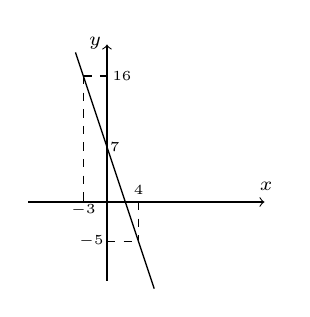
\begin{tikzpicture}[scale=0.1]
\tikzset {line01/.style={line width =0.5pt}}
\tikzset{line02/.style={line width =1pt}}
\tikzset{line03/.style={dashed,line width =0.5pt}}
%\filldraw [black] (0,0) circle (1pt);
\draw [->] (-10,0) -- (20,0);
\draw [->] (0,-10) -- (0,20);
\draw[line01] (-4,19) -- (6,-11);
\draw[line03] (-3,16) -- (0,16);
\draw[line03] (-3,16) -- (-3,0);
\draw[line03] (4,0) -- (4,-5);
\draw[line03] (0,-5) -- (4,-5);
%\draw[line03] (-1,1) -- (0,1);
%\draw[line03] (-1,0) -- (-1,1);
%\draw[line01] (0,-3) -- (-2,5);
%\draw (0.6,-4) node {\tiny $-4$};
%\draw (-1.6,-0.7) node {\tiny $-1$};
\draw (20.2,2) node {\scriptsize $x$};
\draw (-3,-1) node {\tiny $-3$};
\draw (4,1.5) node {\tiny $4$};
\draw (-2,-5) node {\tiny $-5$};
\draw (1,7) node {\tiny $7$};
\draw (1.9,16) node {\tiny $16$};
\draw (-1.5,20.2) node {\scriptsize $y$};
\end{tikzpicture}$$
